\section{Evaluation}

We evaluate Meerkat.Graph in the single-source context-free path querying scenario.
We use a PC with Ubuntu 18.04 installed for evaluation.
It has Intel core i7-6700 CPU, 3.4GHz, and DDR4 32Gb RAM.
The Neo4j database is embedded into the application.

The dataset contains two real-world RDFs: \emph{Geospecies} which contains information about the biological hierarchy\footnote{\emph{Geospecies} RDF: \url{https://old.datahub.io/dataset/geospecies}. Access date: 12.03.2020.} and \emph{Enzyme} which is a part of the UniProt database\footnote{Protein sequences data base: \url{https://www.uniprot.org/}.
RDFs are available here: \url{ftp://ftp.uniprot.org/pub/databases/uniprot/current_release/rdf}. Access date: 12.03.2020.}.
A detailed description of these graphs is presented in the table~\ref{tbl:datasetDetails}.
Note, that the full graphs were loaded into the database by using Neosemantix tool\footnote{Neosemantix is a Neo4j plugin for RDF to Neo4j import. Project page: \url{https://neo4j.com/labs/nsmtx-rdf/}. Access date: 30.03.2020.}, not only the edges labeled by the relations used in queries.

{
\setlength{\tabcolsep}{4pt}
\begin{table}[ht]
\begin{tabular}{|c|c|c|c|c|c|c|c|}
\hline
 Graph      & \#V & \#E & \#SCO & \#T & \#NT & \#BT \\
 \hline
 \emph{Enzyme}     & 15088  & 47953   & 8202 & 15081 & 6819  & 8195 \\
 \emph{Geospecies} & 225134 & 1631525 & 0    & 89062 & 20830 & 20867 \\
 \hline
\end{tabular}
\caption{Details of graphs}
\label{tbl:datasetDetails}
\end{table}
}

\vspace{-0.75cm}

The queries for the evaluation are versions of the same-generation query~---~a classical context-free query useful for hierarchy analysis.
All queries in our evaluation are created using the functions described in section~\ref{sect:combinators}.
Namely, we create and evaluate three queries $Q_1$, $Q_2$ and $Q_3$ as presented below.

\begin{lstlisting}
def q1 (startV) =
    val q =
        sameGen(makeBrs(RDFS__SUB_CLASS_OF ::
                        RDF__TYPE :: Nil))
    queryFromV(startV, q)
\end{lstlisting}

\begin{lstlisting}
def q2 (startV) =
    val q =
        sameGen(makeBrs(SKOS__BROADER_TRANSITIVE :: Nil))
    queryFromV(startV, q)
\end{lstlisting}

\begin{lstlisting}
def q3 (startV) =
    val q =
        sameGen(makeBrs(SKOS__NARROWER_TRANSITIVEY :: Nil))
    queryFromV(startV, q)
\end{lstlisting}

It is plain to see that once the set of appropriate functions is created, new queries can be easily constructed.

We run every query from each vertex of each graph and measure elapsed time and required memory by using ScalaMeter library\footnote{ScalaMeter library Web page: \url{https://scalameter.github.io/}. Access date: 12.03.2020.}.

The results of the evaluation are presented in figures~\ref{fig:time_per_paths_SCO} and~\ref{fig:mem_per_paths_SCO} for query $Q_1$, in figures~\ref{fig:time_per_paths_BT} and~\ref{fig:mem_per_paths_BT} for query $Q_2$, and in figures~\ref{fig:time_per_paths_NT} and~\ref{fig:mem_per_paths_NT} for query $Q_3$.
Note that some results are presented in Appendix~\ref{sec:evlaDetails}.
For each query result size we average the time and memory required, and for each set of points we also draw the linear approximation of this set.
While memory consumption is quite stable, time measurements contain some outliers which are not significant.
We provide a standart boxplot for $Q_3$ in figure~\ref{fig:time_per_paths_NT_boxplot}.

\begin{figure}[ht]
  \begin{center}
    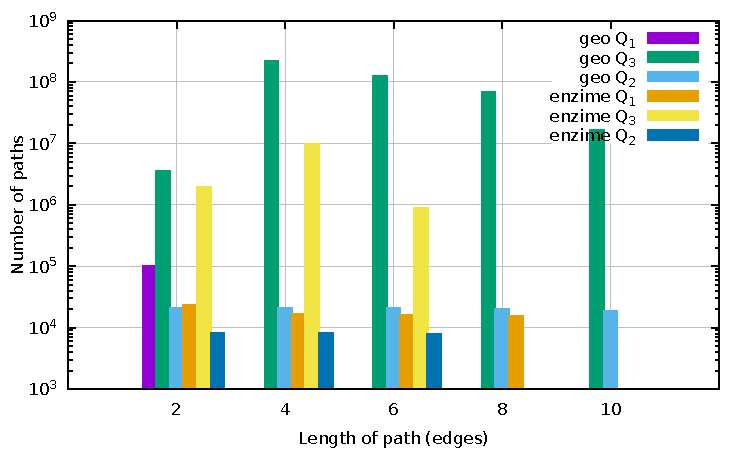
\includegraphics[width=0.5\textwidth]{data/path_per_length.pdf}
    \caption{Paths length distribution}\label{fig:pLength}
  \end{center}
\end{figure}

We also collect the distribution of paths length which shown in figure~\ref{fig:pLength}.
Paths distribution shows that most paths in the queries results are short: the longest consists of 10 edges.

\begin{figure}[ht]
  \begin{center}
    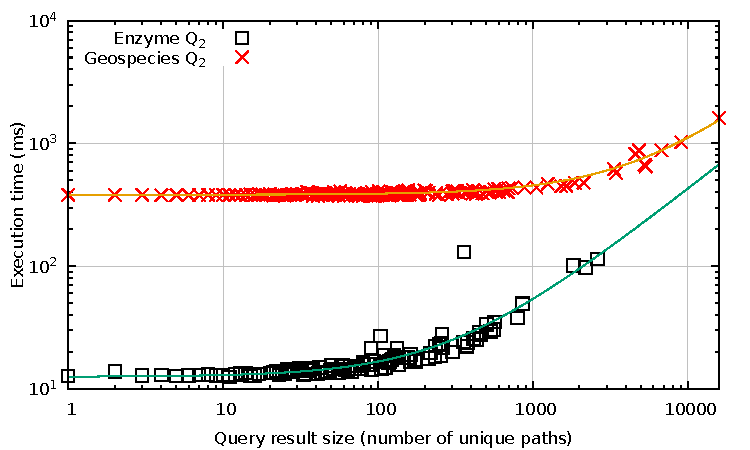
\includegraphics[width=0.5\textwidth]{data/time_per_paths_BT.pdf}
    \caption{Execution time for $Q_2$ query}
    \label{fig:time_per_paths_BT}
  \end{center}
\end{figure}

Figures~\ref{fig:time_per_paths_BT},~\ref{fig:time_per_paths_NT} and~\ref{fig:time_per_paths_SCO} show the dependency of the evaluation time on the query result size (the number of unique paths).
We can see that query evaluation time is linear on result size.
The time required to evaluate a query for one specific vertex is small: for $Q_2$ and \emph{Enzyme} RDF 15051 queries (99.75\%) were executed in less then 20ms, and only 3 queries required more than 100ms.

\begin{figure}[ht]
  \begin{center}
    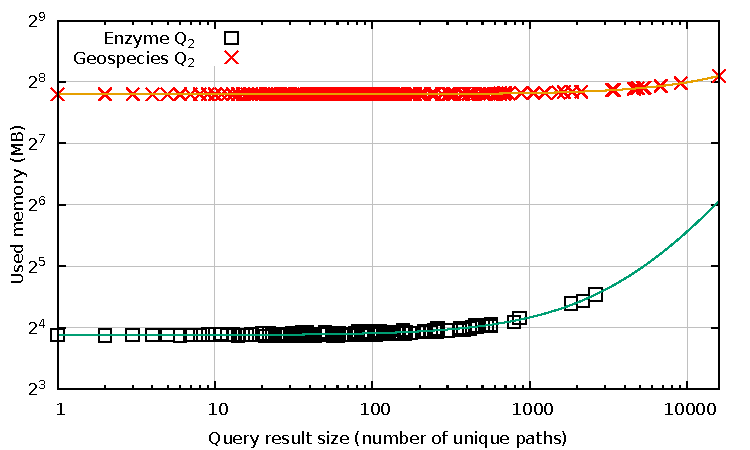
\includegraphics[width=0.5\textwidth]{data/mem_per_paths_BT.pdf}
    \caption{Memory consumption for $Q_2$ query}
    \label{fig:mem_per_paths_BT}
  \end{center}
\end{figure}

Figures~\ref{fig:mem_per_paths_BT},~\ref{fig:mem_per_paths_NT}, and~\ref{fig:mem_per_paths_SCO} show dependency of memory required for the evaluation on the query result size.
We can see, that memory consumption is linear on result size, and is relatively small (does not exceed 512 Mb even for the larger results).

We can see, that both the time and memory consumption depend on the input graph size, and there is a constant overhead independent from the query and the query result size.
We believe the reason to be that Meerket.Graph is implemented on top of Neo4j and thus cannot use internal data structures and create an optimal query execution plan.
For example, it performs a linear scan over all vertices for each query to find the start vertex.
It is the reason for the time difference between runs for the \emph{Enzyme} and \emph{Geospecies} datasets.
To prevent such issues, query execution mechanisms should be deeply integrated into the database engine.

Finally, we can conclude that confext-free path querying in the single-source scenario can be efficiently evaluated in case when the number of paths in the  answer is big but their length is relatively small, while all pairs scenario is still complicated~\cite{10.1145/3335783.3335791}.
We can also see that while the theoretical time and space complexity of CFPQ algorithms is at least cubic, in the scenario demonstrated the real execution time and used memory are linear.
Thus it is necessary to provide detailed time and space complexity analysis of the algorithms.